\documentclass[11pt]{article}
\usepackage[margin=0.6in]{geometry}
\usepackage{mathpazo}
\usepackage{amsmath,amssymb}
\usepackage{microtype}
\usepackage{booktabs}
\usepackage{graphicx}
\usepackage[dvipsnames]{xcolor}
\usepackage{tikz}
\usetikzlibrary{positioning,arrows.meta,calc,fit,backgrounds}
\usepackage[most]{tcolorbox}
\usepackage{enumitem}
\usepackage{listings}
\usepackage[font=small,labelfont=bf]{caption}
\usepackage{hyperref}
\hypersetup{colorlinks=true,linkcolor=MidnightBlue,citecolor=MidnightBlue,urlcolor=MidnightBlue}
\usepackage{cleveref}
\urlstyle{tt}
\def\UrlBreaks{\do\_\do/\do.}
\newcommand{\file}[1]{\nolinkurl{#1}}
\newcommand{\code}[1]{\texttt{#1}}
\newcommand{\mhh}{m_{hh}}
\newcommand{\bw}{\boldsymbol{\omega}}
\newcommand{\bp}{\boldsymbol{p}}
\newcommand{\bx}{\boldsymbol{x}}
\newcommand{\data}{\mathcal{D}}

\definecolor{trainable}{HTML}{1B6CA8}
\definecolor{physics}{HTML}{2E933C}
\definecolor{datac}{HTML}{7B4EA3}
\definecolor{warn}{HTML}{C0392B}

\newtcolorbox{keyidea}[1][]{enhanced,breakable,colback=physics!6,colframe=physics!70!black,
  fonttitle=\bfseries,title={#1},boxrule=0.6pt,arc=2pt,left=6pt,right=6pt}
\newtcolorbox{aside}[1][]{enhanced,breakable,colback=trainable!5,colframe=trainable!70!black,
  fonttitle=\bfseries,title={#1},boxrule=0.6pt,arc=2pt,left=6pt,right=6pt}
\newtcolorbox{assume}[1][]{enhanced,breakable,colback=datac!5,colframe=datac!70!black,
  fonttitle=\bfseries,title={#1},boxrule=0.6pt,arc=2pt,left=6pt,right=6pt}
\newtcolorbox{watch}[1][]{enhanced,breakable,colback=warn!5,colframe=warn!70!black,
  fonttitle=\bfseries,title={#1},boxrule=0.6pt,arc=2pt,left=6pt,right=6pt}
\setlist{itemsep=2pt,topsep=3pt}
\setlength{\emergencystretch}{3em}

\lstset{language=Python, basicstyle=\ttfamily\small, columns=fullflexible,
  keepspaces=true, commentstyle=\color{physics!70!black}\itshape,
  keywordstyle=\color{trainable!90!black}\bfseries, stringstyle=\color{datac},
  showstringspaces=false, frame=single, rulecolor=\color{gray!40},
  backgroundcolor=\color{gray!3}, xleftmargin=4pt, xrightmargin=4pt,
  aboveskip=6pt, belowskip=6pt}

\setlist{itemsep=0pt,topsep=1pt,parsep=0pt}
\pagestyle{plain}
\begin{document}
\begin{center}
{\large\bfseries HEFTNet: modelling the di-Higgs $m_{hh}$ spectrum and its uncertainty}\\[2pt]
{\small P.~Bhat (Fermilab), N.~De~Filippis (Politecnico di Bari),\\
K.\,F.~Johnson, H.\,B.~Prosper, R.~Starnes (Florida State University)}\\[2pt]
{\small Executive summary and roadmap, October 31, 2026}
\end{center}
\vspace{-4pt}
\small
\noindent\textbf{Goal.} A fast surrogate for POWHEG: the cross section per 15~GeV bin of
$m_{hh}$ (255--1455~GeV) as a function of five HEFT coefficients, with a calibrated
uncertainty. \texttt{HEFTNet} writes $\sigma = \sum_{i=1}^{23} C_i(\theta)\,a_i(m_{hh})$, with
known polynomials $C_i$ and 23 functions $a_i$ given by a network of 3,944 parameters that
sees only $m_{hh}$. Training: 3,989 POWHEG spectra (274,152 rows used); validation on 1,000
independent test spectra.

\begin{keyidea}[Principal findings]
\begin{enumerate}[leftmargin=1.3em]
  \item \textbf{The data are exact Poisson counts.} Every spectrum is $q_s \times$ integer
    counts (40,000 generated events per run; a few incomplete runs, listed in \file{data/README.md}). The noise is
    known exactly; the earlier estimate ($N_\text{eff}$) was within 3\% for typical spectra.
  \item \textbf{Weight the errors by the noise.} L1 training leaves the threshold region
    poor ($\langle\chi^2\rangle = 8.4$ per bin at 255--555~GeV). A fine-tune with the Huber
    loss of the pulls ($\delta = 2$) brings it to 1.6 (insensitive to $\delta$), with median
    $\chi^2/N = 1.07$ on the test spectra.
  \item \textbf{The ensemble spread is mostly optimisation, and it under-covers.} 20-network
    ensembles (seeds; bootstrap of rows): 80\% of the fine-tuned spread is due to the
    random seed, 20\% to the finite sample; the spread is 5.6\% of the POWHEG noise, and the
    pulls have s.d.\ 1.07 (1.15 near threshold).
  \item \textbf{The model error dominates.} A discrepancy term $a(m_{hh})\sigma_k^2$, with
    $a = 0.76\,e^{-(m_{hh}-255)/76\,\text{GeV}} + 0.11$ fitted on held-out training rows,
    i.e.\ 0.3--0.9 of the noise, gives pull s.d.\ 1.003 (1.02 near threshold) and
    95.1\% of bins with $|z|<2$ (95.4\% expected).
  \item \textbf{Bayes works, once computed correctly.} HMC (Neal's method) gave a good mean
    but a width of 0.5\% of the noise, because a single chain could not explore a posterior
    with curvature ratios $\sim\!10^6$. A mixture of linearised Laplace approximations about
    the 20 networks (exact for this architecture, 30~s per network on a CPU) gives
    2.4\% (within networks) $\oplus$ 5.6\% (between) $= 6.1\%$ of the noise; the prior
    hardly matters ($\pm4\%$). The posterior is narrow because $\sim$400 effective
    parameters are fixed by $2.8\times10^5$ rows; calibration requires the model-error term.
  \item \textbf{Where the surrogate fails}: the worst test spectra are those with the
    smallest total cross section (strong destructive interference), e.g.\ $\chi^2/N = 68$ at
    the smallest-$\sigma$ test point.
\end{enumerate}
\end{keyidea}

\noindent\textbf{Investigations, in order.}
\begin{itemize}[leftmargin=1.2em]
  \item \emph{BNN with HMC} (\file{hmc.py}): Laplace and Gaussian likelihoods, 10\% and full
    data, longer trajectories; diagnosis in \file{docs/bnn/bnn_plan2.pdf}.
  \item \emph{Ensembles} (\file{ensemble.py}): seeds vs bootstrap, law-of-total-variance
    decomposition, the reference-ensemble question (\file{docs/ensemble}).
  \item \emph{Huber-pull fine-tune} (\file{finetune.py}): $\delta = 1, 2, 3, \infty$;
    10,000 full-batch steps (\file{docs/huber}).
  \item \emph{Exact counts} (\file{counts.py}): scale factor and integer counts per
    spectrum; empty bins restored (\file{docs/counts}).
  \item \emph{Mixture of Laplace approximations} (\file{laplace.py}): MacKay's evidence for
    the prior, linearisation checks (\file{docs/bnn/laplace_explained.pdf}).
\end{itemize}

\noindent\textbf{Recommended result for the paper.} The fine-tuned ensemble mean, with
uncertainty = ensemble spread (or the Laplace mixture) $\oplus$ model error; the Bayesian
mixture as a consistent cross-check. Draft appendix and the 9-panel spectra figure:
\file{docs/paper}.

\noindent\textbf{Open items.} Re-quote the appendix with the exact Poisson noise (shifts of
$\sim$1\%); the model error is treated as independent between bins (a correlated,
Gaussian-process discrepancy is the principled extension); the short POWHEG runs listed in \file{data/README.md} are kept in the default training file;
consider more training points where the cross section is small.

\newpage
\begin{center}
{\large\bfseries The \texttt{dihiggs} repository at a glance}
\end{center}
\vspace{-6pt}
\begin{center}
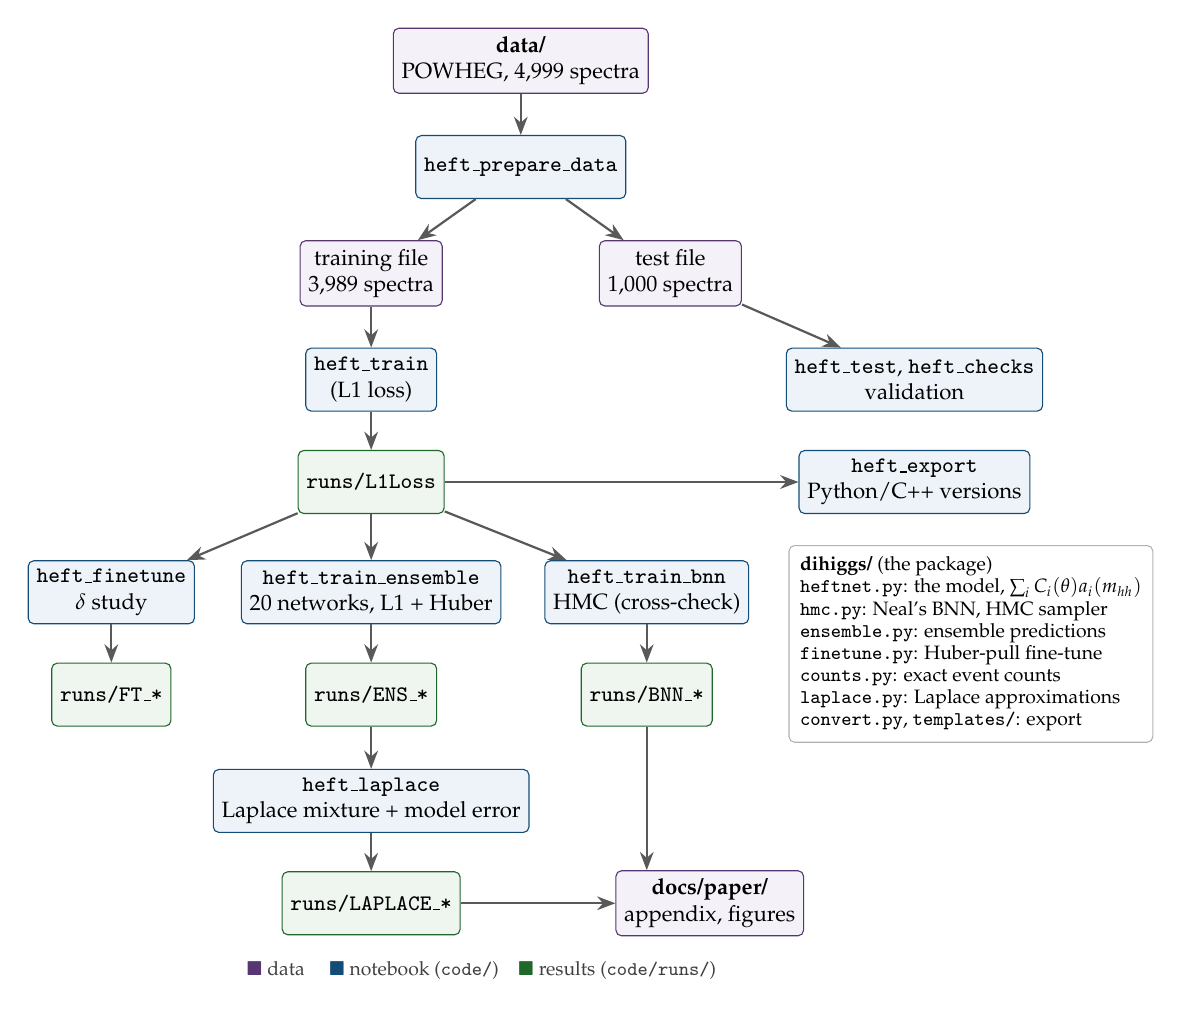
\begin{tikzpicture}[
  font=\footnotesize, >=Stealth,
  dat/.style={draw=datac!70!black, fill=datac!8, rounded corners=2pt, align=center, inner sep=3pt, minimum height=8mm},
  nb/.style={draw=trainable!70!black, fill=trainable!8, rounded corners=2pt, align=center, inner sep=3pt, minimum height=8mm},
  run/.style={draw=physics!70!black, fill=physics!8, rounded corners=2pt, align=center, inner sep=3pt, minimum height=8mm},
  arr/.style={->, thick, gray!70!black}]
  \node[dat] (src) at (0,0) {\textbf{data/}\\POWHEG, 4,999 spectra};
  \node[nb]  (prep) at (0,-1.35) {\texttt{heft\_prepare\_data}};
  \node[dat] (tr) at (-1.9,-2.7) {training file\\3,989 spectra};
  \node[dat] (te) at (1.9,-2.7) {test file\\1,000 spectra};
  \node[nb]  (train) at (-1.9,-4.05) {\texttt{heft\_train}\\(L1 loss)};
  \node[run] (l1) at (-1.9,-5.35) {\texttt{runs/L1Loss}};
  \node[nb]  (ft) at (-5.2,-6.75) {\texttt{heft\_finetune}\\$\delta$ study};
  \node[nb]  (ens) at (-1.9,-6.75) {\texttt{heft\_train\_ensemble}\\20 networks, L1 + Huber};
  \node[nb]  (bnn) at (1.6,-6.75) {\texttt{heft\_train\_bnn}\\HMC (cross-check)};
  \node[run] (ftr) at (-5.2,-8.05) {\texttt{runs/FT\_*}};
  \node[run] (ensr) at (-1.9,-8.05) {\texttt{runs/ENS\_*}};
  \node[run] (bnnr) at (1.6,-8.05) {\texttt{runs/BNN\_*}};
  \node[nb]  (lap) at (-1.9,-9.4) {\texttt{heft\_laplace}\\Laplace mixture + model error};
  \node[run] (lapr) at (-1.9,-10.7) {\texttt{runs/LAPLACE\_*}};
  \node[nb]  (test) at (5.0,-4.05) {\texttt{heft\_test}, \texttt{heft\_checks}\\validation};
  \node[nb]  (exp) at (5.0,-5.35) {\texttt{heft\_export}\\Python/C++ versions};
  \node[dat] (paper) at (2.4,-10.7) {\textbf{docs/paper/}\\appendix, figures};
  \draw[arr] (src) -- (prep); \draw[arr] (prep) -- (tr); \draw[arr] (prep) -- (te);
  \draw[arr] (tr) -- (train); \draw[arr] (train) -- (l1);
  \draw[arr] (l1) -- (ft); \draw[arr] (l1) -- (ens); \draw[arr] (l1) -- (bnn);
  \draw[arr] (ft) -- (ftr); \draw[arr] (ens) -- (ensr); \draw[arr] (bnn) -- (bnnr);
  \draw[arr] (ensr) -- (lap); \draw[arr] (lap) -- (lapr);
  \draw[arr] (te) -- (test); \draw[arr] (l1.east) -- ++(1.2,0) |- (exp.west);
  \draw[arr] (lapr) -- (paper); \draw[arr] (bnnr.south) -- (bnnr.south |- paper.north);
  \node[draw=gray!60, rounded corners=2pt, align=left, inner sep=4pt, anchor=north west, font=\scriptsize] at (3.4,-6.15)
   {\textbf{dihiggs/} (the package)\\
    \texttt{heftnet.py}: the model, $\sum_i C_i(\theta)a_i(m_{hh})$\\
    \texttt{hmc.py}: Neal's BNN, HMC sampler\\
    \texttt{ensemble.py}: ensemble predictions\\
    \texttt{finetune.py}: Huber-pull fine-tune\\
    \texttt{counts.py}: exact event counts\\
    \texttt{laplace.py}: Laplace approximations\\
    \texttt{convert.py}, \texttt{templates/}: export};
  \node[font=\scriptsize, gray!50!black, align=center] at (-0.5,-11.55)
   {\textcolor{datac!70!black}{$\blacksquare$} data \quad
    \textcolor{trainable!70!black}{$\blacksquare$} notebook (\texttt{code/})\quad
    \textcolor{physics!70!black}{$\blacksquare$} results (\texttt{code/runs/})};
\end{tikzpicture}
\end{center}

\vspace{-4pt}
\noindent\textbf{Roadmap of the documents} (all in \file{docs/}; read top to bottom, or jump to the topic you need)
\vspace{2pt}

\noindent{\footnotesize
\begin{tabular}{@{}p{0.30\textwidth}p{0.66\textwidth}@{}}
\toprule
\textbf{Start here} & \\
\file{paper/executive_summary.pdf} & this summary \\
\midrule
\textbf{Physics and the model} & \\
\file{theory.pdf} & LHC Higgs WG note on EFT descriptions of $hh$ production (arXiv:2304.01968): the $C_i$ \\
\file{dihiggs_model.pdf} & the \texttt{HEFTNet} model: exact $\theta$ dependence, a one-dimensional learning problem \\
\file{spectra.pdf} & one-page overview of the POWHEG spectra \\
\midrule
\textbf{Data, pipeline and checks} & \\
\file{report/dihiggs_report.pdf} & the pipeline from POWHEG files to trained and tested model \\
\file{checks_plan.pdf} & three checks of the data and test pipeline \\
\file{counts/counts_note.pdf} & the spectra are scaled Poisson counts: exact noise \\
\midrule
\textbf{Training} & \\
\file{huber/huber_plan.pdf} & the Huber-pull fine-tune (the accuracy gain near threshold) \\
\file{curriculum_plan.pdf}, \file{\_v2.pdf} & side study: curriculum learning \\
\midrule
\textbf{Uncertainty} & \\
\file{ensemble/ensemble_plan.pdf} & seeds and bootstrap ensembles; the reference-ensemble question \\
\file{bnn/bnn_plan.pdf} & design of the Bayesian network and the HMC module \\
\file{bnn/bnn_run1.pdf}--\file{run3.pdf} & the three HMC runs (incl.\ a primer on mixing) \\
\file{bnn/bnn_plan2.pdf} & why HMC gave too-small widths; the Laplace plan \\
\file{bnn/laplace_explained.pdf} & the mixture of Laplace approximations, explained, with results \\
\midrule
\textbf{Paper} & \\
\file{paper/appendix_draft.pdf} & draft JHEP appendix on the uncertainty \\
\file{paper/fig_*.pdf} & paper figures: 9 spectra (\file{fig_spectra_panel}); the 23 $a_i(m_{hh})$ (\file{fig_coefficients}) \\
\file{paper/all_test_spectra.pdf} & all 1,000 test spectra against the model (51 pages) \\
\midrule
\textbf{Practical} & \\
\file{remote_gpu.pdf} & running the notebooks on the RTX 5090 (\texttt{tmux}, \texttt{nohup}) \\
\bottomrule
\end{tabular}}

\end{document}
